\documentclass[a4paper, 12pt]{report}

% Чтобы работала кириллица
\usepackage[T2A]{fontenc}
\usepackage[utf8]{inputenc}

% Делаем человеческие отступы (экономим бумагу)
\usepackage[left=1.3cm,right=1.3cm,top=2cm,bottom=2cm]{geometry}

% Чтобы можно было вставлять кириллицу в формулы
\usepackage{amsmath}

% Вставляем картинки
\usepackage{graphicx}

% Для ссылок во всемирную сеть
\usepackage{nohyperref}  % This makes hyperref commands do nothing without errors
\usepackage{url}  % This makes \url work


% Меняем подпись рисунков и таблиц на русский
\renewcommand{\figurename}{Рис.}
\renewcommand{\tablename}{Табл.}

% Title Page
\title{Лабораторная работа №2\\ Динамическая память}
\author{Зелинский Виктор}
\date{7 мая 2024}


\begin{document}
	\maketitle
	\newpage
	\section*{Увеличивающийся буфер}
	\begin{figure}[h]
		\centering
		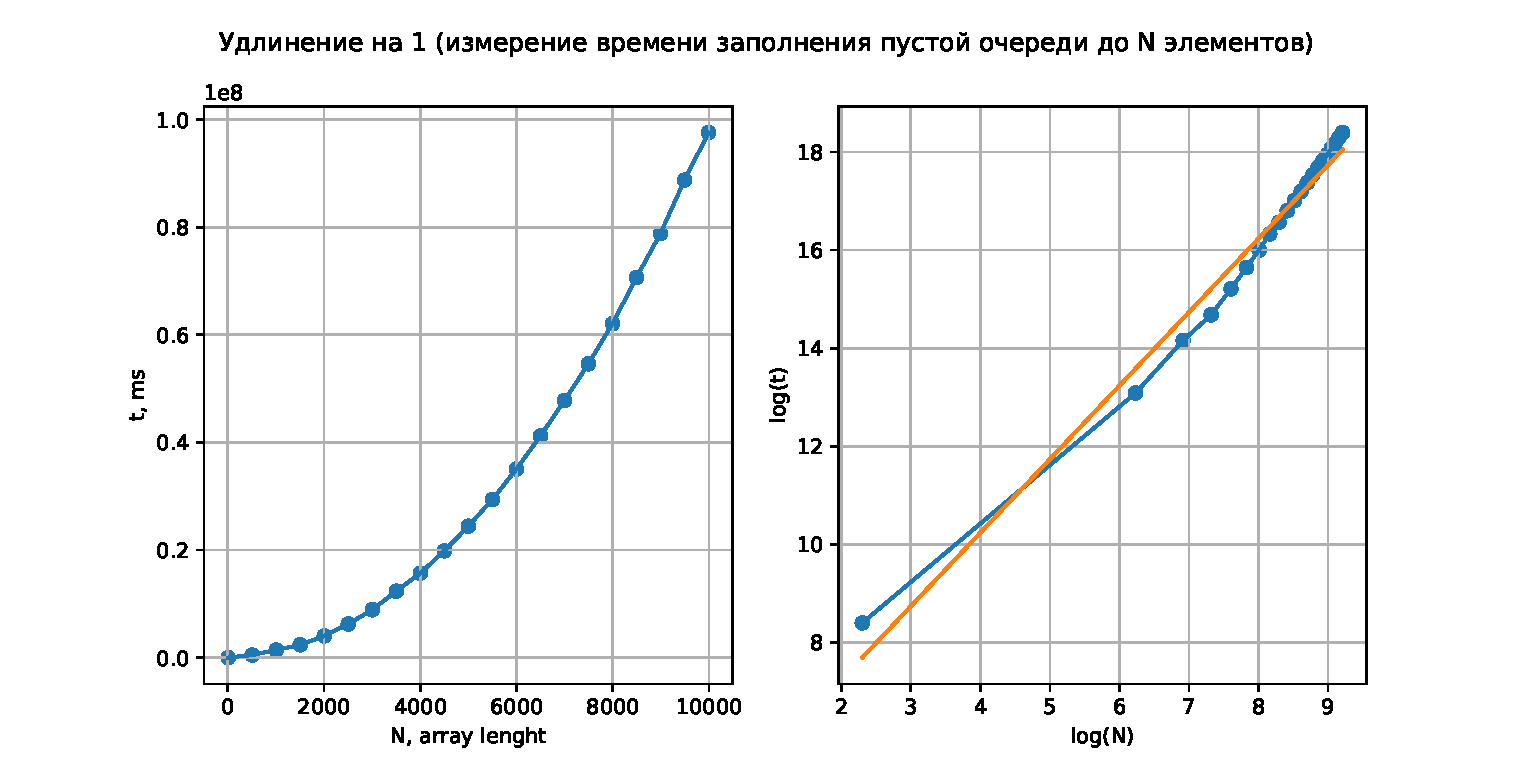
\includegraphics[width=0.6\linewidth]{./oneadd/oneadd.eps}
		\caption{Удлинение на 1}
		\label{fig:oneadd}
	\end{figure}
	
	Коэффициент в МНК = 1.5 (здесь стоило выкинуть первые пару точек, но даже так можно сказать, что сложность $O(N^2)$, тогда сложность добавления одного элемента - $O(N)$) (удлинение на 1 - \figurename \ref{fig:oneadd})
	
	\begin{figure}[h]
		\centering
		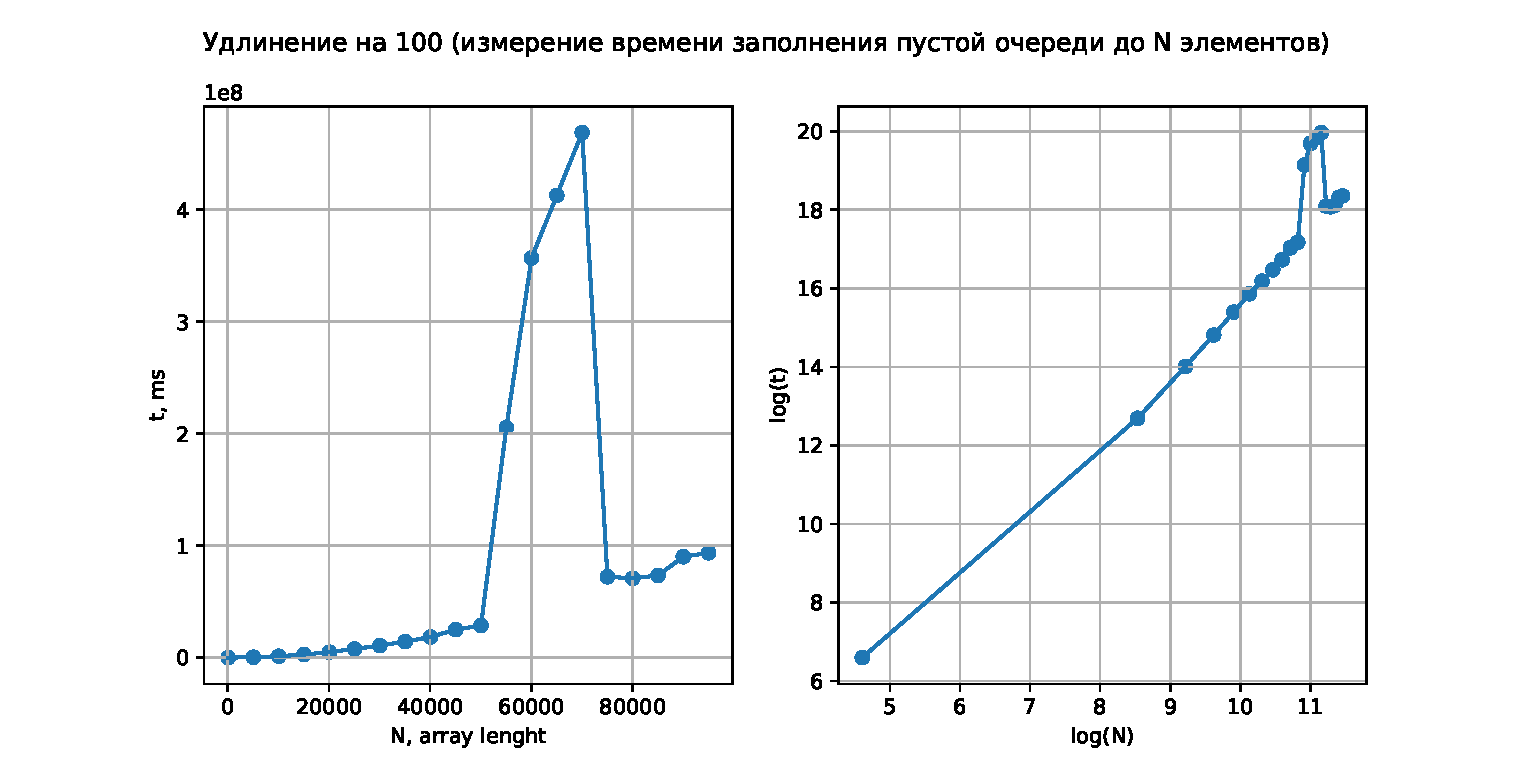
\includegraphics[width=0.6\linewidth]{./cadd/cadd.eps}
		\caption{Удлинение на 100}
		\label{fig:cadd}
	\end{figure}

	Коэффициент в МНК = 1.9, Аналогично предыдущему пункту. (удлинение на 100 - \figurename \ref{fig:cadd})
	
	\begin{figure}[h]
		\centering
		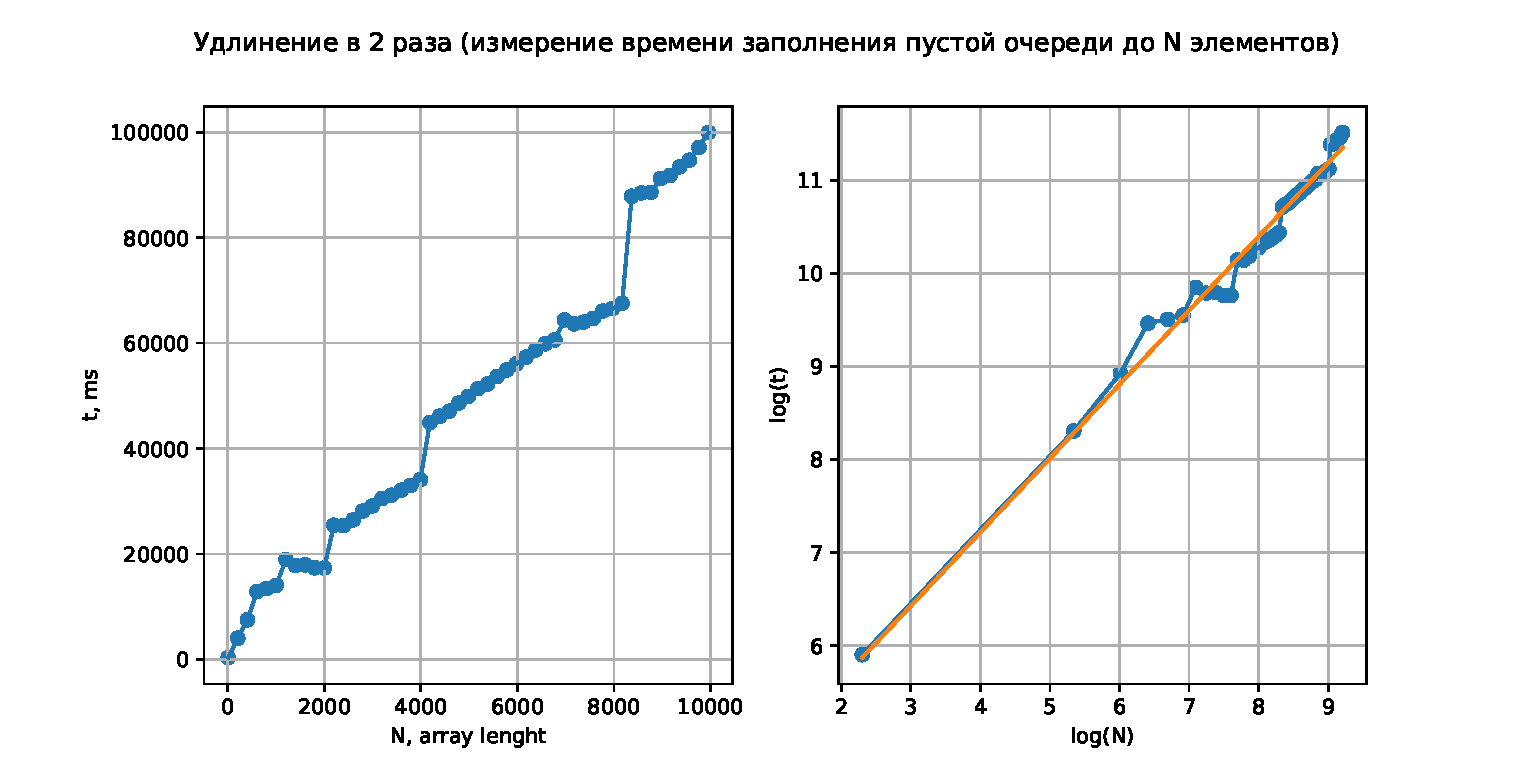
\includegraphics[width=0.6\linewidth]{./multiply/multiply.eps}
		\caption{Удлинение в 2 раза}
		\label{fig:multiply}
	\end{figure}
	
	Коэффициент в МНК = 0.8, а здесь уже $O(1)$ (удлинение в 2 раза - \figurename \ref{fig:multiply})
	\section*{Очередь}
	Метод `push` уже был протестировани в предыдущем пункте, протестируем теперь `poll` (теоретически должно получится O(1), \figurename \ref{fig:poll})
	
	\begin{figure}[h]
		\centering
		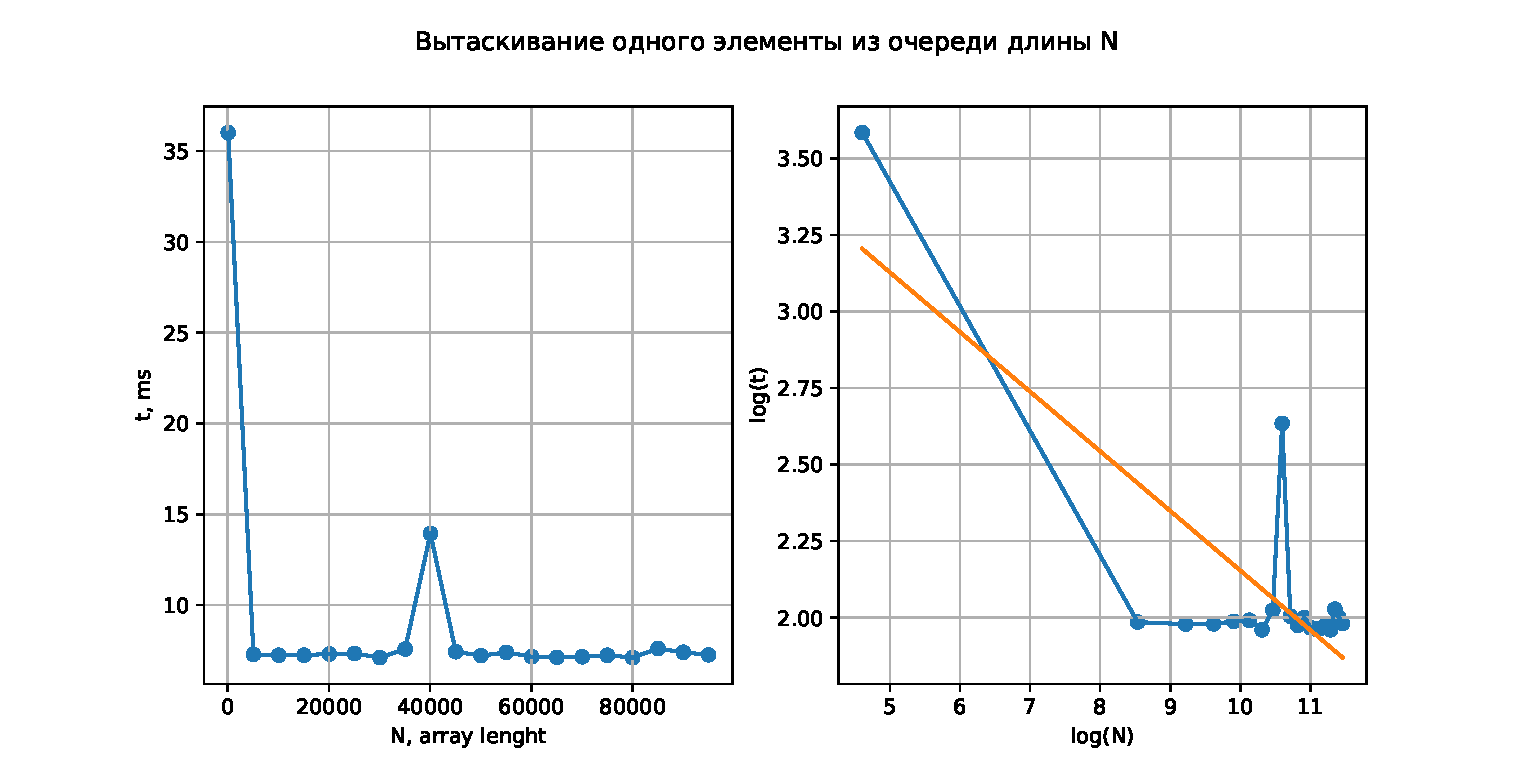
\includegraphics[width=0.6\linewidth]{./queue/poll.eps}
		\caption{Тестирование метода `poll`}
		\label{fig:poll}
	\end{figure}

	Если выбросить первую точку, то это O(1)
\end{document}          
